%%%%%%%%%%%%%%%%%%%%%%%%%%%%%%%%%%%%%%%%%%%%%%%%%%%%%%%%%%
%
% Vzor pro sazbu kvalifikační práce
%
% Západočeská univerzita v Plzni
% Fakulta aplikovaných věd
% Katedra informatiky a výpočetní techniky
%
% Petr Lobaz, lobaz@kiv.zcu.cz, 2016/03/14
%
%%%%%%%%%%%%%%%%%%%%%%%%%%%%%%%%%%%%%%%%%%%%%%%%%%%%%%%%%%

% Možné jazyky práce: czech, english
% Možné typy práce: BP (bakalářská), DP (diplomová)
\documentclass[czech,DP]{thesiskiv}

% Definujte údaje pro vstupní strany
%
% Jméno a příjmení; kvůli textu prohlášení určete, 
% zda jde o mužské, nebo ženské jméno.
\author{Zdeněk Valeš}
\declarationmale

%alternativa: 
%\declarationfemale

% Název práce
\title{Určování nahraditelnosti a\\kompatibility webových služeba}

% 
% Texty abstraktů (anglicky, česky)
%
\abstracttexten{The text of the abstract (in English). It contains the English translation of the thesis title and a short description of the thesis.}

\abstracttextcz{Text abstraktu (česky). Obsahuje krátkou anotaci (cca 10 řádek) v češtině. Budete ji potřebovat i při vyplňování údajů o bakalářské práci ve STAGu. Český i anglický abstrakt by měly být na stejné stránce a měly by si obsahem co možná nejvíce odpovídat (samozřejmě není možný doslovný překlad!).
}

% Na titulní stranu a do textu prohlášení se automaticky vkládá 
% aktuální rok, resp. datum. Můžete je změnit:
%\titlepageyear{2016}
%\declarationdate{1. března 2016}

% Ve zvláštních případech je možné ovlivnit i ostatní texty:
%
%\university{Západočeská univerzita v Plzni}
%\faculty{Fakulta aplikovaných věd}
%\department{Katedra informatiky a výpočetní techniky}
%\subject{Bakalářská práce}
%\titlepagetown{Plzeň}
%\declarationtown{Plzni}

%%%%%%%%%%%%%%%%%%%%%%%%%%%%%%%%%%%%%%%%%%%%%%%%%%%%%%%%%%
%
% DODATEČNÉ BALÍČKY PRO SAZBU
% Jejich užívání či neužívání záleží na libovůli autora 
% práce
%
%%%%%%%%%%%%%%%%%%%%%%%%%%%%%%%%%%%%%%%%%%%%%%%%%%%%%%%%%%

% Zařadit literaturu do obsahu
\usepackage[nottoc,notlot,notlof]{tocbibind}

% Umožňuje vkládání obrázků
\usepackage[pdftex]{graphicx}
\graphicspath{{./img/}}

% Odkazy v PDF jsou aktivní; navíc se automaticky vkládá
% balíček 'url', který umožňuje např. dělení slov
% uvnitř URL
\usepackage[pdftex]{hyperref}
\hypersetup{colorlinks=true,
  unicode=true,
  linkcolor=black,
  citecolor=black,
  urlcolor=black,
  bookmarksopen=true}

% Při používání citačního stylu csplainnatkiv
% (odvozen z csplainnat, http://repo.or.cz/w/csplainnat.git)
% lze snadno modifikovat vzhled citací v textu
\usepackage[numbers,sort&compress]{natbib}
%%%%%%%%%%%%%%%%%%%%%%%%%%%%%%%%%%%%%%%%%%%%%%%%%%%%%%%%%%
%
% VLASTNÍ TEXT PRÁCE
%
%%%%%%%%%%%%%%%%%%%%%%%%%%%%%%%%%%%%%%%%%%%%%%%%%%%%%%%%%%
\begin{document}
%
\maketitle
\tableofcontents

\chapter{Úvod}

- k čemu je práce dobrá
- co text práce obahuje
- use casy

\chapter{Principy webových služeb, techniky}

 - co je to API
 - co jsou to webové služby
 - REST
 - asi by bylo fajn zmínit i XML
 - relevantní protokoly:
 	- HTTP (na REST a obecné API)
 		- protokol aplikační vrstvy
 	- SOAP (web service)
 		- typicky používá HTTP
 		- používá XML pro popis datového modelu
 		- specifikace: https://www.w3.org/TR/soap12-part1/\#intro
 - mohlo by se hodit: https://www.w3.org/TR/2004/NOTE-ws-arch-20040211/\#relwwwrest
 	- popisuje vztah REST a WWW
 			 - REST: založeno na manipulaci s XML reprezentací webových resources skrze stateless operace
 	- popis použitých technologií: XML, SOAP, WSDL
 	- formální popis použití WS
 - popis architektonického stylu REST: https://www.ics.uci.edu/~fielding/pubs/dissertation/rest\_arch\_style.htm
 	- popis elementů:
 		- data, konektory, komponenty
 	- popis view(na modelování)
 - RFC na HTTP: https://tools.ietf.org/html/rfc7231\#section-4
 	- odkaz konkrétně na request methods
 	- mohlo by se hodit, protože ty jsou indexovány, tak alespoň na citaci
 - existují různé, strojově čitelné, formáty pro popis API
 	- WSDL, WADL, JSON-WSP
 	- Swagger, Raml, OpenApi
 	- v případě REST bohužel není nic formálně nutné (oproti třeba SOAP), takže specifikace API nemusí být kompatibilní, nemusí být úplné, nebo můžou být ad-hoc (např. slovní popis ve Word dokumentu) a tím pádem nemusí existovat univerzální způsob strojového čtení těchto specifikací
 
\chapter{Datové typy a porovnávání}

- přednášky z FJP
- jak jazyky řeší datové typy
	- rekurzivní vs. nerekurzivní
- primitivní typy (v xsd)
- built-in typy (v Jave)
- tady budu citovat \cite{abadi1995subytping}
	- subtyping: A <: B <=> A může být použito v kdekoliv kde je očekáváno B
	- kontravariance: F'(A) <: F(B) <=> B <: A

\subsection{Porovnávání datových typů}

 - jak to funguje
 - problémy při porovnání
 - subtyping vs. matching (\cite{abadi1995subytping})


\chapter{Popis ukládání metadat v CRCE, popis indexování API}

Tato kapitola popisuje formát a způsob ukládání metadat v úložišti CRCE. Dále je zde popsána funkce modulů, která indexují API a získané údaje, nad kterými je později provedeno porovnání, ukládají do CRCE.

\section{CRCE}

\begin{itemize}
	\item Citovat \cite{brada2015repository}
	\item CRCE je systém pro ukládání SW komponent, který je vyvíjený na KIV FAV
	\item CRCE je modulární a lze přidat pluginy pro indexaci custom dat
\end{itemize}

\subsection{Metadata v CRCE}

 - Metadata v CRCE mají hierachickou strukturu:
	 - Resource + Capability + Properties + Atributy
	 - taky Requirements, ale ty v práci nepoužívám
	 - Resource reprezentuje indexovanou komponentu
	 - jednotlivé featury (indexovaná data) jsou reprezantovány stromem Capabilit
	 	- k Resource je vždy přiřazena root Capabilita
	 	- každá Capabilita má namespace, podle kterého lze určit co za konkrétní vlastnost popisuje
	 	- v případě root Capability by namespace měl být unikátní pro Resource (a resource by tedy neměl mít více root Capabilit s jedním namespace (snad?))
	 	- detaily fetatury jsou pak uloženy v dětských capabilitách, jejich Properties a Attributes
 - Capability mají Attributy + Properties
 - Properties mají atributy
 - Attributes pak nesou konkrétní hodnoty (Capability a Propeties slouží pouze jako jakési kontejnery)
 - Lze tak modelovat různé vlastnosti indexovaného objektu (viz \cite{brada2015repository}, tam je to dobře popsaný)
 - hierarchická struktura metadat je vhodná pro reprezentaci webových API, která jsou rovněž hierarchická
 
 \begin{figure}[h]
 	\centering
 	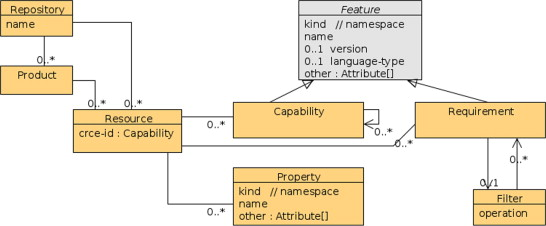
\includegraphics{resource-uml}
 	\caption{Reprezentace metadat v CRCE}
 	\label{fig:crce-resource-uml}
 \end{figure}

\section{Indexování API}
\label{sec:api-index}

- různé druhy jsou jinak indexované
- každý druh API indexován vlastním modulem - diplomky Pejřimovského \cite{pejrimovsky2015ws} a Hessové \cite{hessova2015rest}
- někde by asi bylo fajn ustanovit názvosloví použité v práci:
	- co je API: interface přístupné skrze síť (internet)
	- co je web service: service popsaný WSDL, WADL, nebo Json-WSP dokumentem
	- co je service: Service element in WSDL
	- co je endpoint
		- WSDL: port+operation
		- endpoint: REST, WADL, JSON-WSP
- indexované API je v CRCE uloženo jako Resource		
- popis API je reprezentován jako samostatná feature (1 root Capability) daného Resource
	- Namespacy kořenových Capabilit si definuje indexer
- Service a endpoint jsou reprezentovány jako Capaibility
- endpoint parametry, endpoint response, endpoint request body a endpoint request body jako Property
	- obecná struktura indexovaných dat na obrázku \ref{fig:indexed-api-general}
- vlastní hodnoty pak jako Attribute
- příklad metadat indexovaného API: \ref{fig:indexed-api-example}

\begin{figure}[h]
	\centering
	\caption{Obecná struktura indexovaného API}
	\label{fig:indexed-api-general}
\end{figure}

 \begin{figure}[h]
	\centering
	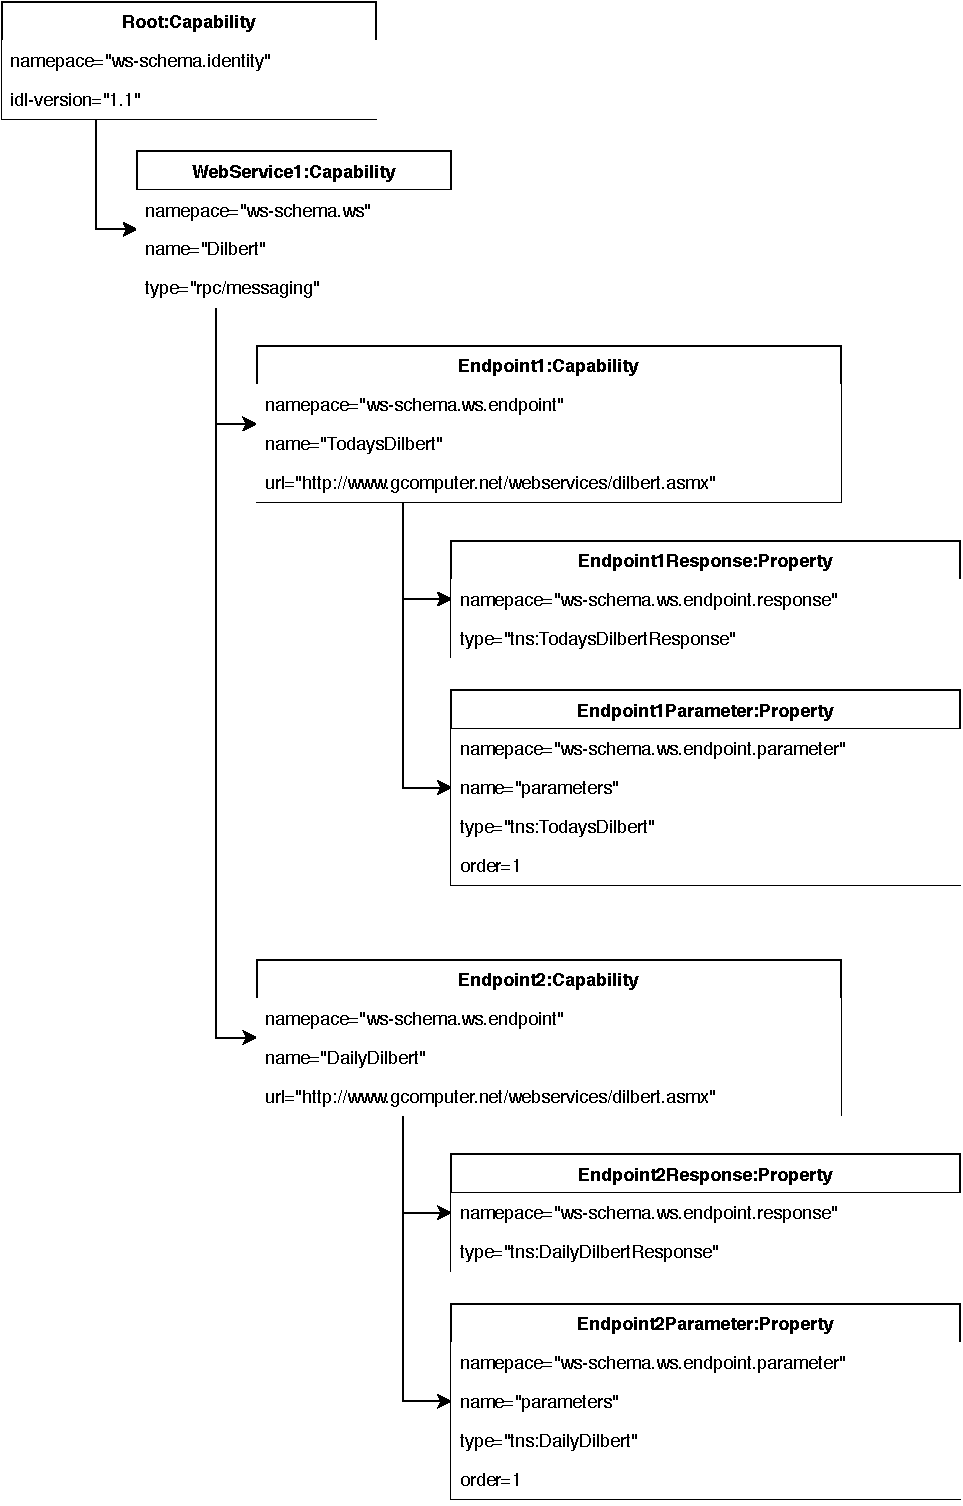
\includegraphics[height=13cm]{indexed-api-example}
	\caption{Příklad indexované SOAP web service Dilbert }
	\label{fig:indexed-api-example}
\end{figure}

\subsection{Indexování REST API}

- práce: \cite{hessova2015rest}
- binární analýza JAR s implementací API
- funguje na principu hledání patternů v byte kódu
- indexer vytváří hierarchii metadat ve formátu root capability -> child endpoint capabilities
- podpora formátů:
	- REST: JAX-RS, Spring Web MVC podporovány

\subsection{Indexování WS}

- práce: Pejřimovského \cite{pejrimovsky2015ws}
- nějaký trefný obrázek indexovaných dat
- konkrétní formát API detekován z buď z formátu vstupního souboru, nebo z metadata v top elementech
- podle typu je pak použit daný parser
- podpora formátů:
	- WSDL: hierarchie root capability -> web service capabilities -> child endpoint capabilities
	- WADL, Json-WSP: hierarchie root capability -> child endpoint capabilities
	- parsování souboru s popisem API, CRCE stačí i URL
- indexer obsahoval drobné chyby, které jsem v rámci DP opravil
	- špatná indexace URL v případě WSDL (nebyla podle specifikace)

\subsection{Limity indexování}

 - custom datové typy
 - 2 problémy
	- rekurzivní typy
		- jsou způsoby pro jejich rozvoj: \cite{abadi1995subytping} a ukládání
		- nicméně indexovací logika není implementovaná (ani v jednom ze zmíněných indexerů)
	- chybějící definice custom typů
		- v případě např REST jsou uloženy v implementaci (nemusí se jednat ani o stejnou knihovnu) a indexer k nim nemusí mít přístup
		- tím pádem je jméno datového typu (např. fully qualified name v případě Java třídy) jedinou informací, která je o typu dostupná

\chapter{Popis funkce porovnávače (co se jak porovnává pro jaké typy API)}

V této kapitole je detailně popsána funkce porovnávacího algoritmu společně s daty, nad kterými je možné porovnávač použít. Zároveň je zde popsán způsob vyhodnocení výsledků porovnání a formát takto získaných dat.

\section{Popis porovnávacího algoritmu}

Porovnávací algoritmus pracuje s výše zmíněnými metadaty, reprezentovanými stromovou strukturou, jejíž uzly tvoří instance tříd \verb|Capability|, \verb|Properties| a \verb|Attributes|. Algoritmus pracuje pouze s daty, která byla vytvořena indexery popsanými v části \ref{sec:api-index}. Ostatní metadata, jež mohou být případně navěšená na \verb|Resource| reprezentující API zůstanou nedotčena. V současné době je možné porovnat pouze API, jejichž metadata byla vytvořena stejným indexerem. Není tedy možné porovnat například metadata REST API získaná binární analýzou jar s metadaty získanými čtením JSON-WSP dokumentu.

- zmínit taky omezení, která plynou z indexovaných dat

\subsection{Složitost algoritmu}

- v nejhorším případě:

	- WSDL: $O(n^3)$ (ws endpointy ve ws)
	
	- ostatní $O(n^2)$ (endpointy1 x endpointy 2)

\subsection{Obecný algoritmus porovnání}

TODO: obecný popis, formulovat lépe

Algoritmus pro vše krom WSDL obecně (WSDL má navíc výběr a porovnání webservice):
\begin{enumerate}
	\item Vstupem jsou endpointy obou API: \verb|endpoints1|, \verb|endpoints2|
	\item Vyber endpoint \verb|e1| z \verb|endpoints1|
	\item Vyber endpoint \verb|e2| z \verb|endpoints2|, který je vhodný k porovnání s \verb|e1|
	\item Pokud neexistuje vhodný \verb|e2|, ulož mezivýsledek reprezentující přebývající endpoint a jdi zpět na 2
	\item Postupně porovnej metadata, parametry, tělo request, tělo response obou endpointů
	\item Ulož objekt reprezentující mezivýsledek porovnání
	\item Pokud není \verb|endpoints1| prázdné, jdi na krok 2, jinak pokračuj dále
	\item Pro všechny zbývající endpointy \verb|endpoints2| ulož mezivýsledek reprezentující chybějící endpoint
	\item Z mezivýsledků sestav finální objekt reprezentující výsledek porovnání dvou API
\end{enumerate}

\subsection{Problémy při porovnávání}	

TODO: rozepsat v patřičných subsections
\begin{enumerate}
	\item jak vybrat který endpoint/ws porovnat s kterým
	\item MOV - pick the best
	\item datové typy (java built-in, xsd, custom)
	\item verze v URL u REST API (taky vede na MOV)
\end{enumerate}
	
\subsubsection{Výběr endpointu/ws vhodného k porovnání}

Metadata:
\begin{itemize}
	\item kvůli MOV se teoreticky nelze spoléhat na jméno endpointu
	\item kvůli verzi v cestě k endpointu (popsáno dále v \ref{sec:api-path-version}) se nelze spoléhat na cestu k endpointu
\end{itemize}

Počet parametrů
\begin{itemize}
	\item některé mohou být nepovinné
\end{itemize}
 
\subsubsection{Porovnávání datových typů}
Custom datové typy: nejsou indexované a lze tedy porovnávat pouze podle jména (např fully qualified name v případě Java tříd).
 
Built-in datové typy (java, xsd)

\begin{itemize}
	\item Java: podpora typů z \verb|java.lang| + dědičnost
	\item xsd: podpora built-in typů xsd (musí být správná předpona) + dědičnost ve smyslu 'vejde se do'
\end{itemize}

	
\subsubsection{Verze REST API v cestě k endpointu}	
\label{sec:api-path-version}

Proč: 

\begin{itemize}
	\item klient může chtít volat novou verzi API a je tedy žádané zjistit, jak moc je API kompatibilní (např. se mohla změnit jen implementace, takže signatura je stále stejná)
	
	\item Normálně by algoritmus skončil MUT, protože by kvůli rozdílným cestám k endpointům vyhodnotil endpointy z API 1 jako DEL a endpointy z API 2 jako INS
	
	\item to není žádané, takže algoritmus je schopný detekovat verzi v cestě k endpointu a při výběru endpointů k porovnání ji ignorovat
\end{itemize}

Podporovaný formát:
\begin{itemize}
	\item \verb|v<major>[.minor[.micro]]|
	\item lowecase i uppercase
	\item oddělovač může být '.', nebo '-'
	\item regex: \verb|\/[vV][0-9]+(?:[.-][0-9]+){0,2}\/|
\end{itemize}

Detekci verze je možno vypnout. Pokud je detekce zapnutá, algoritmus se před porovnáním cest pokusí najít verzi a pokud ji najde, z cesty ji vyřadí a porovná cesty bez verze
	
\subsection{MOV flag}	

Popis MOV

Co: Příznak označující, že API/endpoint má (částečně) shodnou implementaci, ale nachází se na jiné adrese

Proč: endpointy v API mohou mít jiné url/jména, ale implementačně mohou být shodné -> potřeba detekovat

Jak: na základě ostatních metadat (počet parametrů, počet endpointů ve WS)

Mov se také nastaví pokud je zaplé ignorování verzi REST API v endpoint path a pokud: 
\begin{itemize}
	\item cesty s verzí nejsou stejné
	\item cesty bez verze jsou stejné
\end{itemize}

Algorimuts (nemusí vždy fungovat správně):
\begin{itemize}
	\item  obecná detekce před samotným porovnáním -> MovDetectionResult
	\item  3x diff: host, path to endpoint, operace
	\item  MovDetectionResult se pak použije při výběru endpointu k porovnání a při samotném porovnání (pickBest)
\end{itemize}
	
- kombinace které vedou na mov: 
\begin{itemize}
	\item $h \land !pe \land !o$
	\item $h \land pe \land !o$
	\item TODO
\end{itemize}
	
	
\section{Výsledek porovnání - Diff}	
Popis výsledné datové struktury
\begin{itemize}
	\item Diff, Compatibility
	\item vychází z \cite{brada2006diff}
	\item stromová struktura rozdílů mezi jednotlivými uzly stromu metadat
	\item obrázek \ref{fig:diff-construction} hezky popisuje jak to vznikne
	\item výsledné hodnoty diffu a jejich významy pro klienta v tabulce \ref{tab:diff-level}
	\item SPE/GEN může vzniknout jen z daových typů parametrů/response -> lze spolehlivě použít kontravarianci a výsledek obrátit
	\item pokud tedy vyjde SPE, znamená to např generalizovaný parametr a tedy je to pro klienta bezpečné
\end{itemize}
	
\begin{figure}[h]
	\centering
	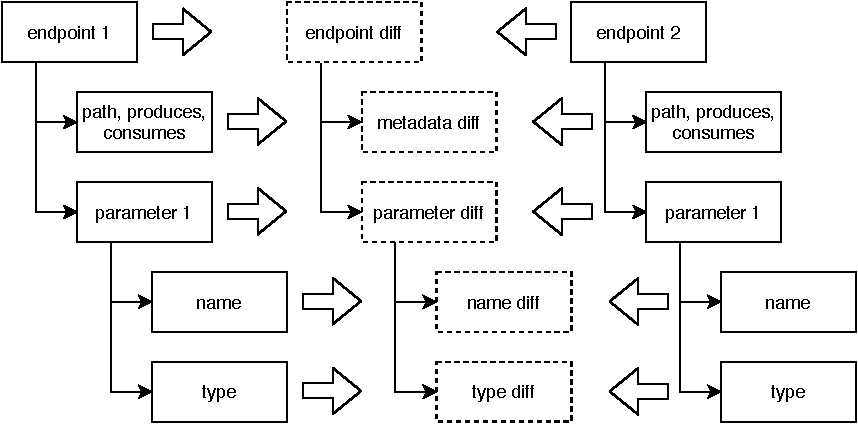
\includegraphics{diff-construction}
	\caption{Vytvoření diffů}
	\label{fig:diff-construction}
\end{figure}

\subsection{Vyhodnocení výsledku}

- jak probíhá vyhodnocení (nejdříve se určí hodnoty listů, z nich se pak počítá dál nahoru)

- kontravariance

	- není to úplně problém, ale při vyhodnocování finálního Diffu pro endpoint je potřeba brát v potaz 
	
	- GEN/SPE může vzniknout jen z datových typů parametrů/response endpointu, takže je to poměrně přímočaré

\begin{table}[h!]
	\centering
	\begin{tabular}{c|c}
		Difference type & Impact on client  \\
		\hline
		None (NON) & safe \\
		Specialization (SPE) & safe  \\
		Insertion (INS) & safe \\
		Deletion (DEL) & potentially dangerous \\
		Generalization (GEN) & potentially dangerous \\
		Mutation (MUT) & dangerous \\
		Unkown (UNK) & dangerous
	\end{tabular}
	\caption{Types of differences between two nodes }
	\label{tab:diff-level}
\end{table}

\chapter{Implementační detaily (jen stručně)}

 - zmínit, proč třídy pro porovnávání REST API a WS nemají společného předka (krom rozhraní)
 	- důvod: chtěl jsem nechat implementaci obou porovnávačů oddělenou pro případ, že by se změnila funkce indexerů

\chapter{Testování}

- nějaká reálná data
	- STAG (WSDL)
	- Fuel Economy
- i syntetická data
- algoritmus testován pomocí unit testů

\section{Integrační + akceptační testy}

- testování skrze REST API
- pomocí Postman (Collection Runner)
- několik verzí jednoho API -> testování křížem
- todo: příklad
	- popsat verze API (čím se liší), případně zdůvodnit očekávaný výsledek
	- tabulka vzájemného porovnání s výsledky

\chapter{Závěr}	

 
% 
% PRO ANGLICKOU SAZBU JE NUTNÉ ZMĚNIT
% CITAČNÍ STYL!
%
\bibliographystyle{csplainnatkiv}
{\raggedright\small
\bibliography{literatura}
}

\end{document}
